\documentclass[a4paper,12pt]{report}

\usepackage[a4paper]{geometry}
\usepackage{amssymb,amsmath,amsthm}
\usepackage{graphicx}
\graphicspath{ {./images} }
\usepackage{url}
\usepackage{hyperref}
\usepackage{epsfig}
\usepackage[italian]{babel}
\usepackage{setspace}
\usepackage{tesi}
\usepackage{makeidx}
\usepackage{caption, float}
\usepackage{subfig}
\usepackage{indentfirst}
\usepackage{algorithmic}
\usepackage{listings,xcolor}

% per le accentate
\usepackage[utf8]{inputenc}

\begin{document}
% per json
\lstset{
	string=[s]{"}{"},
	stringstyle=\color{blue},
	comment=[l]{:},
	commentstyle=\color{black}
}

\setcounter{secnumdepth}{5}
\setcounter{tocdepth}{5}

\title{Un'applicazione web per dimostrare le proprietà degli algoritmi di label propagation}
\author{Andrei Georgiani TALPALARU}
\dept{Corso di Laurea in Informatica} 
\anno{2019-2020}
\matricola{942824}
\relatore{Prof. Paolo CERAVOLO}
\correlatore{Dr. Samira MAGHOOL}

\beforepreface
\prefacesection{Ringraziamenti}
Ringrazio molto il Professore Paolo Ceravolo per avermi permesso di lavorare su questo progetto, da cui ho imparato tante nuove tecnologie su cui non ho avuto modo di mettere mano fino ad ora. 

Ringrazio la mia famiglia, i miei amici e colleghi, che mi hanno sostenuto e aiutato per tutto questo tempo.
\afterpreface
% 
% 
%		
\chapter{Introduzione}

\section{Motivazioni}
L'applicazione è stata sviluppata per permettere agli utenti di vedere il modo in cui funziona l'algoritmo in una maniera visiva e di poter eseguire l'algoritmo in un modo più facile per gli utenti non esperti.

Eseguendo l'algoritmo su più reti si può vedere il modo in cui AVPRA funziona e il fatto che l'iterazione finale e molto vicina al diametro della rete. Entrambe le informazioni (iterazione finale e diametro della rete) sono visibili nell'applicazione e permettono quindi di capire facilmente quanto sono vicini i due valori.

\pagebreak

\section{Divisione Documento}
Il documento e diviso in quattro capitoli:
\begin{itemize}
\item il primo capitolo introduce la nozione di \textbf{Social Network Analysis}, definisce alcuni termini usati spesso in questo ambito, descrive il Label Propagation e dà una descrizione dell'algoritmo su cui si basa il progetto descritto di seguito nel documento.

\item il secondo capitolo offre una comparazione tra l'applicazione sviluppata e altre applicazioni simili per poi andare a descrivere le tecnologie con cui è stata sviluppata l'applicazione. Il capitolo finisce presentando e descrivendo il funzionamento dell'applicazione.

\item il terzo capitolo parla del modo in cui l'applicazione potrebbe evolvere nel futuro e del modo in cui l'applicazione può essere resa disponibile attraverso il deployment.

\item l'ultimo capitolo descrive le conclusioni a cui sono arrivato dopo il sviluppo dell'applicazione.

\end{itemize}
%/
%

\chapter{Social Network Analysis}
	La Social Network Analysis è l'analisi delle strutture sociali attraverso le reti e la teoria dei grafi. \cite{snaintro}
	Grazie ad una rappresentazione astratta, dove le connessioni tra certi elementi di un sistema, chiamati anche nodi o agenti (quando sono capaci di fare scelte o azioni attive), la SNA può essere applicata a una varietà di domini. Il comportamento del sistema, in termini di comunicazione, propagazione ed evoluzione delle connessioni è catturato da metriche di SNA. \cite{avpra}

	\section{Reti}
	Una rete è composta da due componenti di base: i nodi e gli archi. Usando questi due componenti si possono descrivere una moltitudine di strutture e relazioni (per esempio connessioni sociali, connessioni in una rete di computer, reti elettriche \dots). 

	 I nodi sono le entità presenti nella rete e che possono avere proprietà interne (per esempio un valore che rappresenta il grado del nodo, o il peso o una posizione nella rete). 

	Gli archi sono le connessioni tra i nodi che possono avere a loro volta delle proprietà (per esempio un peso o un altro tipo di relazione tra i nodi collegati alle estremità dell'arco).	\cite{snaintro} 

	\section{Comunità}
	Una proprietà fondamentale di molte reti è la struttura a comunità, che rappresenta la tendenza dei nodi di essere aggregati in gruppi distinti, o \textbf{comunità}, in modo che gli archi tra nodi appartenenti alla stessa comunità sono densi, ma gli archi tra nodi appartenenti a comunità diverse sono sparsi. \cite{gregory}

	\section{Label Propagation}
	Label Propagation rappresenta una famiglia di algoritmi usati per predire le etichette dei nodi di una rete. 
	Differisce da altri algoritmi di Social Network Analysis siccome, invece di adottare una visione globale della rete, le decisioni prese dall'algoritmo sono fatte rispetto a proprietà locali, quindi gli algoritmi di Label Propagation adottano una visione locale della rete. \cite{raghavan} 

	L'idea generale è che le etichette assegnate inizialmente ai nodi sono propagate attraverso la rete seguendo gli archi. La propagazione di un'etichetta a un nodo si basa sulle etichette dei suoi vicini, tipicamente ad un salto di distanza. Molteplici iterazioni permettono il raggiungimento di un'approssimazione del ottimo globale partendo da un ottimo locale. La complessità temporale varia tra tempo lineare ed esponenziale, dipendendo dalla densità della rete. L'approccio è naturalmente decentralizzato, con passaggi singoli su ogni nodo ad ogni iterazione. \cite{avpra}
	
	\section{Algoritmi di Label Propagation}
	La scelta principale che differenzia i diversi algoritmi di Label Propagation è legata alla funzione di aggiornamento. Alcune varianti della funzione di aggiornamento che sono state usate nel tempo sono: il grado dei nodi, il coefficiente di clustering e la similarità strutturale.

	La limitazione principale degli algoritmi precedenti era l'impossibilita di scegliere più di un'etichetta per ogni nodo. 

	Gli algoritmi sono stati generalizzati per permettere l'identificazione di comunità sovrapposte. Ogni etichetta viene pesata con un belonging coefficient associato al nodo. 

	\section{Belonging Coefficient / Coefficiente di appartenenza}
	Il belonging coefficient (o coefficiente di appartenenza) indica quanto forte è l'appartenenza di un nodo $x$ a una comunità. Tutti i coefficienti di un nodo sommano a 1. \cite{gregory}

	\section{AVPRA}
	AVPRA (o Agent-based Vector-label PRopagation Algorithm) è un'algoritmo di Label Propagation basato su un'organizzazione ad agenti che permette di implementare la regola di aggiornamento rispetto a più fattori, come per esempio le proprietà di dominio. 

	AVPRA differisce dagli altri algoritmi tramite il fatto che l'output dell'algoritmo è un vettore compatibile col formato di input usato in maggior parte degli algoritmi di \textbf{Machine Learning}. Il vettore ha una lunghezza fissata per tutti i nodi e include tutte le etichette della rete assieme al loro coefficiente di appartenenza (basato sulle proprietà strutturali della rete).

	Il coefficiente di appartenenza nel caso dell'algoritmo AVPRA è una misura di diffusione/accumulo delle etichette dei nodi, dipendente dalla distanza rispetto ad altri nodi e dalla loro frequenza. \cite{avpra} 

		\subsection{Propagazione basata su agenti}
		Consideriamo che le etichette possono scorrere nella rete e che gli agenti possono tenere conto della frequenza di queste. Gli agenti sono semi-intelligenti e agiscono rispetto alla situazione riscontrata. Possono adottare diverse strategie nella ricezione o rifiuto di un'etichetta che scorre da un nodo vicino, in concordanza con certe condizioni. In questo modo, l'algoritmo può controllare gli effetti globali, come per esempio la condizione di terminazione.

		\subsection{Aggiornamento sincrono}
		Per evitare i conflitti nella propagazione degli aggiornamenti, in AVPRA gli agenti sono aggiornati in modo \textbf{sincrono}. Il vettore delle etichette di un certo nodo a tempo $t$ sarà ottenuto dai vettori delle etichette dei vicini a tempo $t-1$. In questo modo tutti gli agenti possono aggiornarsi simultaneamente.
	
		\subsection{Inizializzazione}
		Ogni agente viene etichettato con un vettore di $d$ dimensioni dove $d$ è la cardinalità dell'insieme delle etichette uniche nella rete notato $L$. Ogni posizione di un vettore di etichette di un nodo $x$ viene assegnata a un'etichetta dell'insieme $L$ e nel vettore di etichette vengono memorizzati i coefficienti d'appartenenza del nodo $x$ rispetto a tutte le etichette. 
		
		L'unico requisito dell'inizializzazione è che i vettori di etichette assegnati ai nodi della rete riflettano proprietà reali dei nodi che agiscono come agenti. \cite{avpra}

		\subsection{Funzione di aggiornamento}
		La regola di aggiornamento mostra il modo in cui i vettori di etichette sono aggiornati ad ogni iterazione. In AVPRA, la funzione di aggiornamento è la seguente:
		
		\begin{equation}
		VL_i [l] (t) = w_1 VL_i [l] (t-1) + w_2 \sum_{j \in \Gamma(i)} VL_j [l](t-1)
		\end{equation}

		Dove $VL_i[l](t)$ rappresenta il valore del coefficiente di appartenenza dell'etichetta $l$ nel nodo $n_i$ al tempo $t$, $w_1$ rappresenta il peso delle etichette assegnate al nodo $n_i$ a tempo $t - 1$, $w_2$ rappresenta il peso delle etichette assegnate ai nodi $\Gamma(i)$ a tempo $t - 1$ e $\Gamma(i)$ è l'insieme dei vicini del nodo $n_i$. \cite{avpra}

		\subsection{Algoritmo}

		\begin{algorithmic}
			\REQUIRE Matrice di adiacenza $A_{i, j}$, attributi iniziali in vettori di etichette di $d$ dimensioni per ogni agente

			\FOR{$t$ in Tempi}

				\STATE \COMMENT{Iterazione su tutti gli agenti $i$ della rete}

				\FOR{$i$ in $A_{i, j}$}
					
					\STATE \COMMENT{Iterazione su ogni etichetta del agente $i$}

					\FOR{$k$ in $VL_i$}

						\STATE \COMMENT{Se $j$ e un vicino di $i$, si esegue la funzione di aggiornamento}

						\IF{$A_{i, j}$ == 1}
							\STATE $VL_i[k] = FunzioneAggiornamento(VL_i[k], VL_j[k])$

						\ENDIF
					\ENDFOR
				\ENDFOR	
			\ENDFOR
		\end{algorithmic}

		\subsection{Iterazione Finale}
		L'algoritmo AVPRA finisce quando il sistema raggiunge un'iterazione $s$ nella quale tutti i vettori di etichette sono rimasti stazionari per almeno un numero fissato di iterazioni prima. Il stazionamento implica che le variazioni dei coefficienti di appartenenza devono essere minori di un parametro $p$ che viene chiamato soglia di trascuramento.  \cite{avpra}

		La varianza ad un tempo $t$ (dove $t > 0$) per un nodo $i$ si calcola usando la formula seguente:
		
		\begin{equation}
			Var_i(t) = \frac{\sum_{l \in Ettichete} (VL_i[l](t) - VL_i[l](t-1))}{k}
		\end{equation}

		Dove $k$ rappresenta il numero di etichette uniche della rete, $Ettichete$ e l'insieme di etichette della rete e $VL_i[l](t)$ e il valore del coefficiente di appartenenza dell'etichetta $l$ al nodo $i$ a tempo $t$.

		Nell'esempio sottostante si può osservare come l'iterazione finale è la 4 siccome la variazione tra i vettori di etichette dell'iterazione 4 e quelli dell'iterazione 3 e minore della soglia di trascuramento (di $0.1$ in questo caso), e siccome lo stazionamento è avvenuto anche nelle 2 iterazioni anteriori.
		\begin{center}
			\begin{figure}[H]
				\centering
				\subfloat[\centering Vettore etichette del nodo 1 a tempo 0]{{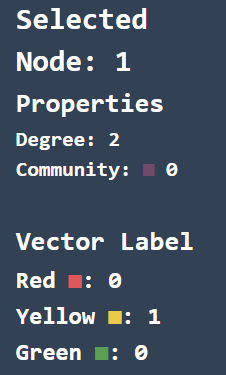
\includegraphics[width=0.2\linewidth,keepaspectratio]{node1vlt0}}}
				\qquad
				\subfloat[\centering Vettore etichette del nodo 2 a tempo 0] {{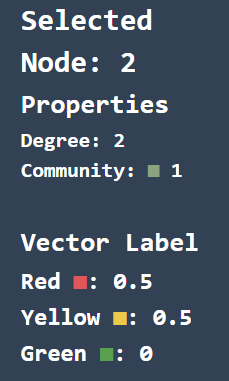
\includegraphics[width=0.2\linewidth,keepaspectratio]{node2vlt0}}}
				\qquad
				\subfloat[\centering Vettore etichette del nodo 3 a tempo 0]{{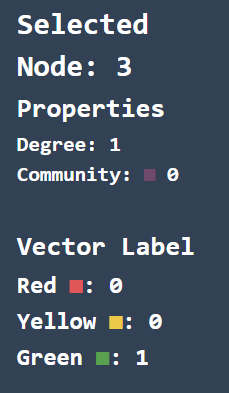
\includegraphics[width=0.2\linewidth,keepaspectratio]{node3vlt0}}}
				\qquad
				\subfloat[\centering Vettore etichette del nodo 4 a tempo 0]{{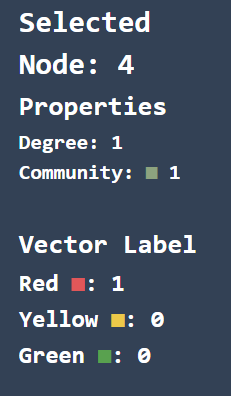
\includegraphics[width=0.2\linewidth,keepaspectratio]{node4vlt0}}}

				\caption{Vettori di etichette a tempo 0}
			\end{figure}
		\end{center}

		\begin{center}
			\begin{figure}[H]
				\centering
				\subfloat[\centering Vettore etichette del nodo 1 a tempo 1]{{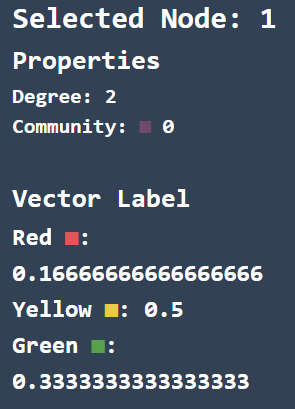
\includegraphics[width=0.2\linewidth,keepaspectratio]{node1vlt1}}}
				\qquad
				\subfloat[\centering Vettore etichette del nodo 2 a tempo 1] {{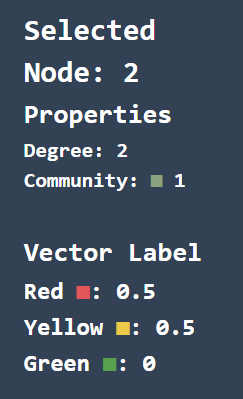
\includegraphics[width=0.2\linewidth,keepaspectratio]{node2vlt1}}}
				\qquad
				\subfloat[\centering Vettore etichette del nodo 3 a tempo 1]{{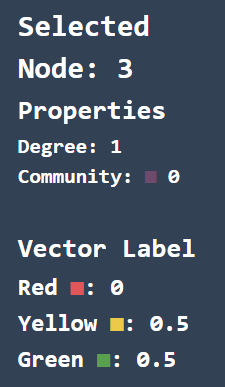
\includegraphics[width=0.2\linewidth,keepaspectratio]{node3vlt1}}}
				\qquad
				\subfloat[\centering Vettore etichette del nodo 4 a tempo 1]{{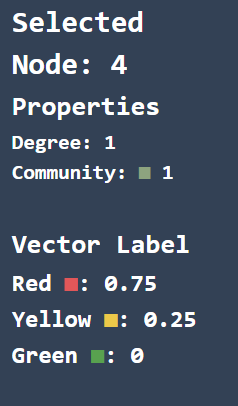
\includegraphics[width=0.2\linewidth,keepaspectratio]{node4vlt1}}}

				\caption{Vettori di etichette a tempo 1}
			\end{figure}
		\end{center}

		\begin{center}
			\begin{figure}[H]
				\centering
				\subfloat[\centering Vettore etichette del nodo 1 a tempo 2]{{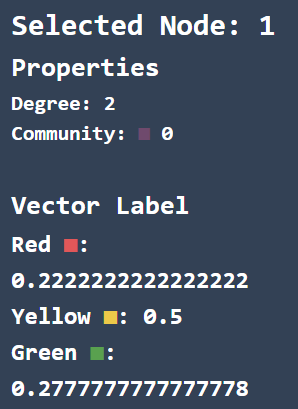
\includegraphics[width=0.2\linewidth,keepaspectratio]{node1vlt2}}}
				\qquad
				\subfloat[\centering Vettore etichette del nodo 2 a tempo 2] {{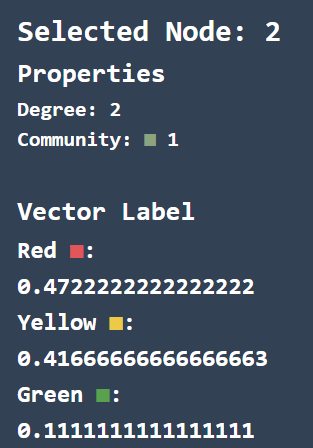
\includegraphics[width=0.2\linewidth,keepaspectratio]{node2vlt2}}}
				\qquad
				\subfloat[\centering Vettore etichette del nodo 3 a tempo 2]{{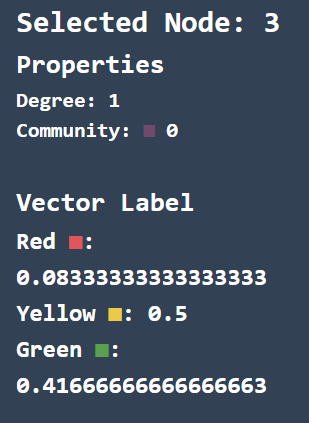
\includegraphics[width=0.2\linewidth,keepaspectratio]{node3vlt2}}}
				\qquad
				\subfloat[\centering Vettore etichette del nodo 4 a tempo 2]{{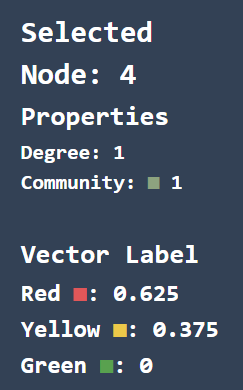
\includegraphics[width=0.2\linewidth,keepaspectratio]{node4vlt2}}}

				\caption{Vettori di etichette a tempo 2}
			\end{figure}
		\end{center}

		\begin{center}
			\begin{figure}[H]
				\centering
				\subfloat[\centering Vettore etichette del nodo 1 a tempo 3]{{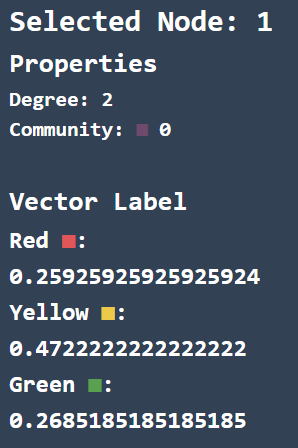
\includegraphics[width=0.2\linewidth,keepaspectratio]{node1vlt3}}}
				\qquad
				\subfloat[\centering Vettore etichette del nodo 2 a tempo 3] {{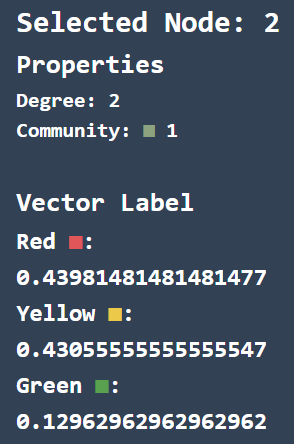
\includegraphics[width=0.2\linewidth,keepaspectratio]{node2vlt3}}}
				\qquad
				\subfloat[\centering Vettore etichette del nodo 3 a tempo 3]{{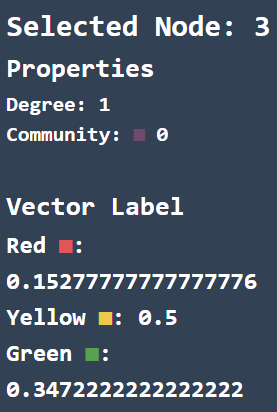
\includegraphics[width=0.2\linewidth,keepaspectratio]{node3vlt3}}}
				\qquad
				\subfloat[\centering Vettore etichette del nodo 4 a tempo 3]{{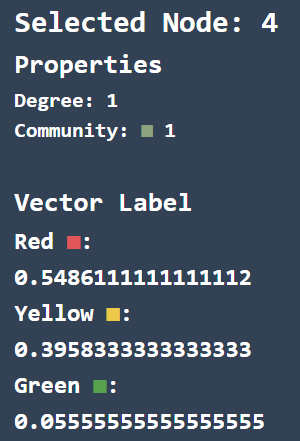
\includegraphics[width=0.2\linewidth,keepaspectratio]{node4vlt3}}}

				\caption{Vettori di etichette a tempo 3}
			\end{figure}
		\end{center}


		\begin{center}
			\begin{figure}[H]
				\centering
				\subfloat[\centering Vettore etichette del nodo 1 a tempo 4]{{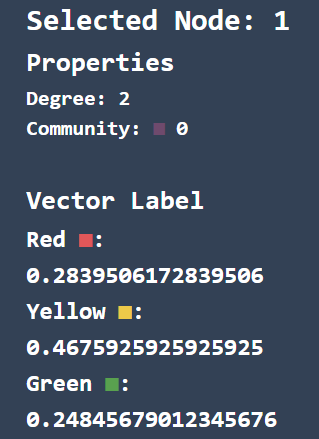
\includegraphics[width=0.2\linewidth,keepaspectratio]{node1vlt4}}}
				\qquad
				\subfloat[\centering Vettore etichette del nodo 2 a tempo 4] {{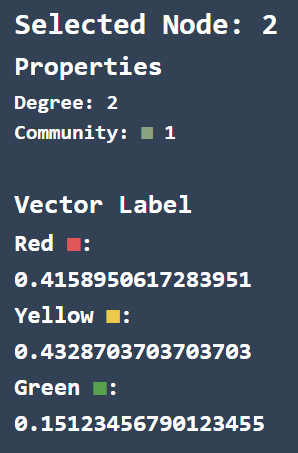
\includegraphics[width=0.2\linewidth,keepaspectratio]{node2vlt4}}}
				\qquad
				\subfloat[\centering Vettore etichette del nodo 3 a tempo 4]{{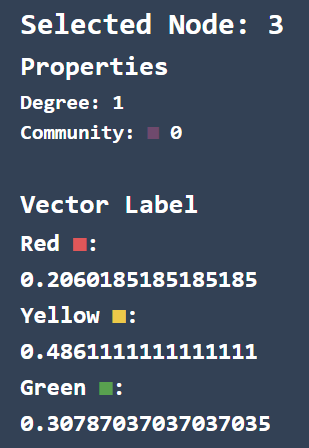
\includegraphics[width=0.2\linewidth,keepaspectratio]{node3vlt4}}}
				\qquad
				\subfloat[\centering Vettore etichette del nodo 4 a tempo 4]{{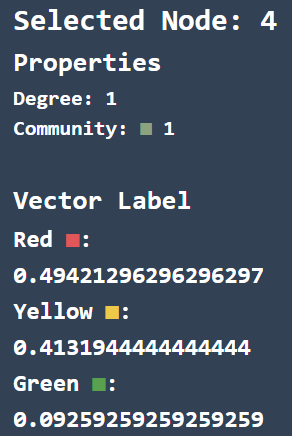
\includegraphics[width=0.2\linewidth,keepaspectratio]{node4vlt4}}}

				\caption{Vettori di etichette a tempo 4}
			\end{figure}
		\end{center}

		Il numero ottimale di iterazioni per la terminazione dell'algoritmo è molto vicino al diametro della rete. Nel esempio presentato, il diametro della rete è 3 e il tempo finale è 4, quindi il numero di iterazioni necessarie per la terminazione dell'algoritmo è 4, molto vicino al diametro 3.

\chapter[Lo sviluppo dell'applicazione]{Lo sviluppo di un'applicazione per dimostrare le proprietà dell'algoritmo AVPRA}

	\section{Applicazioni di visualizzazione delle reti sociali}
		Tra le poche applicazioni che visualizzano reti sociali è stato deciso di confrontare l'applicazione creata con un'altra che si comporta in modo simile, ma che non ha la capacita di eseguire l'algoritmo AVPRA sulle reti visualizzate.

		Per ogni applicazione presa in studio viene data una piccola descrizione ed in seguito vengono elencati \textbf{I Pro} ed \textbf{I Contro} di ogni una.

		\subsection{Visualizzatore Reti Sociali con AVPRA}
		AVPRA è un algoritmo di Label Propagation basato su Agenti.
		Il visualizzatore delle Reti Sociali per AVPRA è un'applicazione web che permette all'utente di
		eseguire e visualizzare i risultati dell'algoritmo in un modo interattivo nel browser web.
		
			\subsubsection*{I Pro}
				\begin{itemize}
					\item Ha tanti parametri che permettono all'utente di controllare il comportamento dell'algoritmo e dell'input.
					\item Permette l'esportazione della rete e delle informazioni visibili sullo schermo in formato PNG.
					\item Permette di esportare le informazioni riguardanti il grafo e il output in formato JSON.
					\item Singoli nodi possono essere selezionati in modo da poter vedere più dettagli e misure riguardanti quel specifico nodo.
					\item Offre la possibilità di selezionare, comparare ed esportare la comparazione tra due nodi diversi della rete.
					\item Sopporta la visualizzazione di due viste diverse: Vector Label View (mostra in modo grafico la distribuzione delle label su ogni nodo) e Community View (mostra in modo grafico la divisione della rete in comunità basate sulla struttura.).
					\item Mostra graficamente la divisione in comunità raggruppando i nodi della stessa comunità più vicini uno all'altro.
					\item Permette all'utente di eseguire l'algoritmo per più iterazioni e di vedere graficamente l'evoluzioni dei Vector Label nel tempo (feature specifica di AVPRA).
					\item La paletta di colori utilizzata per i label nei Vector Label può essere modificata usando un'ulteriore file nella fase di caricamento della propria rete.
					\item Permette all'utente di selezionare un nodo specifico tramite una barra di ricerca dove si può inserire l'id del nodo.
				\end{itemize}
						
			\subsubsection*{I Contro}
				\begin{itemize}
					\item Sopporta un solo formato di input (tre file CSV: Lista Archi, Vector Label Iniziali, Nomi Label) e due formati di output (un file pickled contenente i risultati di tutte le iterazioni dell'algoritmo e un file JSON contenente i dati della rete o la comparazione di due nodi diversi).
					\item I dataset dell'utente e i risultati delle esecuzioni dell'algoritmo su quei dataset sono tenute sul server dell'applicazione, anche se per poco tempo.
					\item Performance più scarse nel caso venga usato con reti molto grandi.
				\end{itemize}

		\subsection{Infomap Network Navigator}
		Infomap è un'algoritmo di clustering su reti basato su Map Equation. Infomap Online è un'applicazione web che permette agli utenti di eseguire
		l'algoritmo Infomap nel browser web. \cite{mapequationsite} 
		
		Infomap Network Navigator è un'applicazione che permette di visualizzare i risultati
		dell'algoritmo in un modo interattivo. \cite{mapequationnavigatorsite} 
		
			\subsubsection*{I Pro}
				\begin{itemize}
					\item I dataset dell'utente e i risultati dell'esecuzione dell'algoritmo su quei dataset non sono mantenute sul server di Infomap Online.
					\item Ha tanti parametri per controllare il comportamento dell'algoritmo, dell'input, del output e dell'accuratezza.
					\item Sopporta tanti formati di input (Link-List, Pajek, Bipartite, Multilayer, With inter-layer links, Without inter-layer links, States) e tanti formati di output (Phyisical, State-level output, Tree, FTree, Clu, Newick, JSON). Infomap riconosce automaticamente il formato dei file dal header del file.
					\item Permette di esportare la visualizzazione in formati SVG e PNG.
					\item Permette l'esportazione del file di output.
					\item Singoli nodi possono essere selezionati in modo da vedere più dettagli e misure riguardati il specifico nodo.
					\item Permette all'utente di selezionare un nodo specifico tramite una barra di ricerca.
					\item Mostra graficamente il raggruppamento dei nodi in comunità e sotto-comunità attraverso un modulo (feature specifica Map Equation).
				\end{itemize}			

			\subsubsection*{I Contro}
				\begin{itemize}
					\item L'esportazione della visualizzazione non include nient'altro oltre la rete stessa.
					\item Non offre la possibilità di vedere il modo in cui due nodi diversi della rete siano correlati.
					\item Esiste un limite sulla dimensione dei file di input che si possono utilizzare.
					\item Non esiste un modo per personalizzare la paletta di colori che viene usata nella visualizzazione.
				\end{itemize}

	\section{Sviluppo}
		Il progetto è un'applicazione web che è divisa in 2 parti:
		\begin{itemize}
		\item Frontend - la componente dell'applicazione con cui l'utente interagisce direttamente.
		\item Backend - la componente dell'applicazione con cui il frontend interagisce e che si occupa di esporre un'API che esegue le funzionalità richieste dal frontend.
		\end{itemize}
		
		\subsection{Funzionalità previste}
			\subsubsection{Backend}
			\begin{itemize}
				\item Dev'essere capace di eseguire l'algoritmo AVPRA dato in Python.
				\item Deve esporre un'API che:
				\begin{itemize}
					\item permette all'utilizzatore di eseguire l'algoritmo.
					\item permette all'utilizzatore di controllare i parametri dell'algoritmo come numero di iterazioni, soglia di trascuramento, interpretazione della rete (diretto, non diretto), modo di propagazione delle label (da predecessori, da successori) e formula dei pesi della regola di aggiornamento.
					\item permette di ottenere i dettagli riguardanti un solo nodo ad una certa iterazione.
					\item permette di ottenere i dettagli riguardanti la relazione tra due nodi ad una certa iterazione.
					\item permette di esportare i risultati e i dettagli dell'esecuzione in un formato definito.
					\item Deve permettere all'utente di caricare ed eseguire l'algoritmo sulla propria rete usando un formato definito.
				\end{itemize}
			\end{itemize}

			\subsubsection{Frontend}
				\begin{itemize}
					\item Deve permettere all'utente di visualizzare in modo interattivo la situazione, alla iterazione corrente, della rete e dei suoi vector label.
					\item Deve implementare un modo in cui l'utente possa caricare la sua propria rete.
					\item Deve dare la possibilità all'utente di avere più informazioni riguardo lo stato corrente di un vector label di un nodo specifico.
					\item Deve permettere di avere informazioni riguardo l'iterazione corrente e l'iterazione finale (da definire) dell'algoritmo.
					\item Deve implementare un modo in cui si possa andare avanti e indietro tra le iterazioni in modo da vedere l'evoluzione dei vector label.
					\item Deve fare possibile la visualizzazione delle comunità associate alla rete.
					\item Deve permettere di selezionare 2 nodi e di vedere la situazione corrente di entrambi.
					\item Deve implementare un modo di esportare i file che si possono esportare attraverso l'API esposta dal backend.
				\end{itemize}

		\subsection{Sviluppo dell'applicazione web}

			\subsubsection{Frontend}
			Per lo sviluppo della parte Frontend dell'applicazione, contenente l'interfaccia utente e la comunicazione col backend, sono state utilizzate diverse tecnologie e librerie. \par
			Le librerie e tecnologie che sono state utilizzate sono presentate di seguito.

			\paragraph*{React.js} \par è una libreria di JavaScript che viene usata per creare in modo facile delle interfacce utente interattive. 
				I componenti più importanti di questa libreria che sono utilizzati all'interno dell'applicazione sono presentati di seguito:
				
				\begin{itemize}
				\item \textbf{Componenti}

				I componenti sono le parti che permettono di organizzare l'interfaccia utente in React. Questi possono essere definiti in due modi: Classi Componente e Funzioni Componente. \cite{componentireact} 

				Le \textbf{Funzioni Componente} sono funzioni JavaScript che prendono in input dei dati (chiamati props) e ritornano degli elementi React che descrivono, tramite JSX, il modo in cui dovrebbe essere visualizzato sullo schermo. \cite{tipicomponenti} 

				Le \textbf{Classi Componente} sono classi che estendono \textbf{React.Component} e che implementano un metodo \textbf{render} che restituisce un elemento React. 

				\item \textbf{Stato} 

				Gli aggiornamenti della UI in JavaScript base dovevano accadere trovando l'elemento nel DOM e aggiornandolo manualmente. React, invece, aggiorna automaticamente l'interfaccia utente in base allo stato interno del componente. 

Prima dell'aggiunta dei Hooks, per modificare il stato interno di un componente era necessario che esso venga scritto come Classe Componente. Dopo l'aggiunta del hook \textbf{useState}, il stato poteva essere utilizzato anche all'interno di una Funzione Componente. 

È necessario usare \textbf{useState} (Funzione Componente) o \textbf{setState} (Classe Componente) in modo che React capisca che l'interfaccia utente che usa il stato interno debba essere renderizzato nuovamente per mostrare il valore aggiornato dello stato. \cite{statoreact} 

				\item \textbf{Hooks} 

				Gli Hooks sono stati aggiunti per permettere di utilizzare stato e altre funzioni che esistevano nelle Classi Componente anche nelle Funzioni Componente \cite{hooksreact}. Alcuni esempi di hooks maggiormente utilizzati sono: 

				\begin{itemize}
				\item \textbf{useState} - hook che permette di aggiungere stato a funzioni componente.
				\item \textbf{useEffect} - hook che permette di aggiungere side effects in funzioni componente, il che significa poter far succedere qualcosa in base al cambiamento delle dipendenze dichiarate. Può essere usato anche per simulare i comportamenti \textbf{componentDidMount} e \textbf{componentDidUpdate} delle classi componenti.

				\end{itemize}
				
				All'interno dell'applicazione sono stati creati alcuni hook che hanno permesso di facilitare il processo di sviluppo. 

				I hook che sono stati implementati sono:
				\begin{itemize}
				\item \textbf{useGUIControls} che mette a disposizione le funzioni e i dati da utilizzare per i controlli delle pagine riguardanti la visualizzazione dei grafi.
				
				\item \textbf{usePolling} che permette di chiamare un endpoint dell'API in modo ripetuto e a intervalli regolari nel caso esso risponde con un codice di \textbf{Not Ready}.
				
				\item \textbf{useSS} che permette di fotografare il schermo e viene utilizzato nel caso in cui si preme il tasto di Screenshot sull'applicazione.			
				\end{itemize}				

				\item \textbf{JSX}

				JSX rappresenta un'estensione di JavaScript che permette di scrivere HTML direttamente all'interno di JavaScript. Usando Babel, JSX viene poi compilato in chiamate \textbf{React.createElement()}. Ciò significa che JSX può essere usato anche in strutture condizionali, per poter produrre risultati diversi rispetto a una decisione. \cite{jsxreact} 

				\end{itemize}
			\paragraph*{Typescript} è un'estensione di JavaScript che aggiunge una sintassi per i tipi e una migliore integrazione coi editor, aiutando in questo modo il sviluppatore a trovare velocemente gli errori dovuti ai tipi. \cite{typescript} 

				I tipi di dati che TypeScript introduce sono:
				\begin{itemize}
				\item number - numero floating point con doppia precisione
				\item string
				\item bigint
 				\item boolean
				\item symbol
				\item null
				\item undefined
				\item object
				\item void - tipo inteso come tipo di ritorno per le funzioni che non ritornano un valore
				\item T[] - array mutabili
				\item {[T, T]} - tuple di dimensione fissata, ma mutabili
				\item (t: T) U - funzioni che prendono in input un tipo T e restituiscono un tipo U
				\end{itemize}

			\paragraph*{Next.js} è un framework di React che risolve maggior parte dei problemi che si incontrano quando si cerca di lavorare solo con la libreria React. Per framework si intende che Next.js gestisce in modo autonomo gli strumenti e le configurazioni che React necessita, offrendo pero anche funzionalità aggiuntive. \cite{nextjs} 

			\paragraph*{D3.js} è una libreria per manipolazione di documenti in base a dati. D3.js permette di associare dati al DOM e costruire visualizzazioni per quei dati sull'applicazione che si sta creando. Nel caso presente D3.js viene utilizzato per costruire la visualizzazione del grafo e per aggiungere interattività ad esso. \cite{d3js} 

			\paragraph*{Katex} è una libreria JavaScript usata per visualizzare formule matematiche sulla pagina. Nel caso presente, questa libreria è stata usata per poter mostrare all'utente la formula coi pesi che si stanno inserendo quando si usa la visualizzazione delle reti personalizzate. \cite{katex} 

			\paragraph*{Tailwind CSS} è un framework di CSS che offre classi di utilità che aiutano il sviluppatore a evitare di scrivere CSS direttamente. Usando solo Tailwind CSS si può evitare di usare valori arbitrari per maggior parte delle misure, e quindi si arriva ad essere più consistenti col design dell'applicazione. Nell'applicazione presentata, questo framework è stato usato per fare tutto il layout del sito. \cite{tailwindcss} 

			\subsubsection{Backend}

			Per lo sviluppo della parte backend dell'applicazione, contenente l'API che ha la capacita di rispondere alle richieste del frontend, sono state utilizzate diverse tecnologie e librerie.

			Le librerie e tecnologie che sono state utilizzate sono presentate di seguito.
			
			\paragraph*{Flask} è un microframework web basato su Python che è stato usato, nel caso presente, per il sviluppo del Backend come un REST API. \cite{flaskforeword}

				Flask permette di creare un’API nel modo più semplice possibile, ed è stato scelto come tecnologia di Backend poiché l'algoritmo che viene usato per la elaborazione delle reti è scritto in Python, e quindi la scelta più facile per un linguaggio di Backend era Python. 

				Nel caso dell'esempio dei colori, il server di backend risponde puramente da file statici con la rete già processata. Nel caso degli esempi personali, i file necessari vengono caricati sul server, vengono processati, e fino alla scadenza della sessione, si può visualizzare la rete personalizzata.

			\paragraph*{Sympy} è una libreria di Python per l'interpretazione di matematica simbolica. È stato usato per poter interpretare le formule per i pesi che vengono mandate dal Frontend nel caso di esempi personalizzati. \cite{sympy}

			\paragraph*{CDlib} è una libreria che aggrega tanti algoritmi di community detection. È stato utilizzato solamente per l'implementazione dell'algoritmo di community detection di Leiden. \cite{cdlib}
			
		\subsection{Presentazione applicazione}
			
			\subsubsection{Pagina Principale}
			La pagina principale serve per permettere all'utente di scegliere tra due modi di diversi di provare e visualizzare i risultati dell'algoritmo. Ogni modo ha una piccola descrizione del come funziona e un tasto per andare alla pagina specifica per quella modalità. Ogni modalità sarà descritta in dettaglio nelle sezioni successive.

			\begin{center}
			\begin{figure}[H]
			\centering
			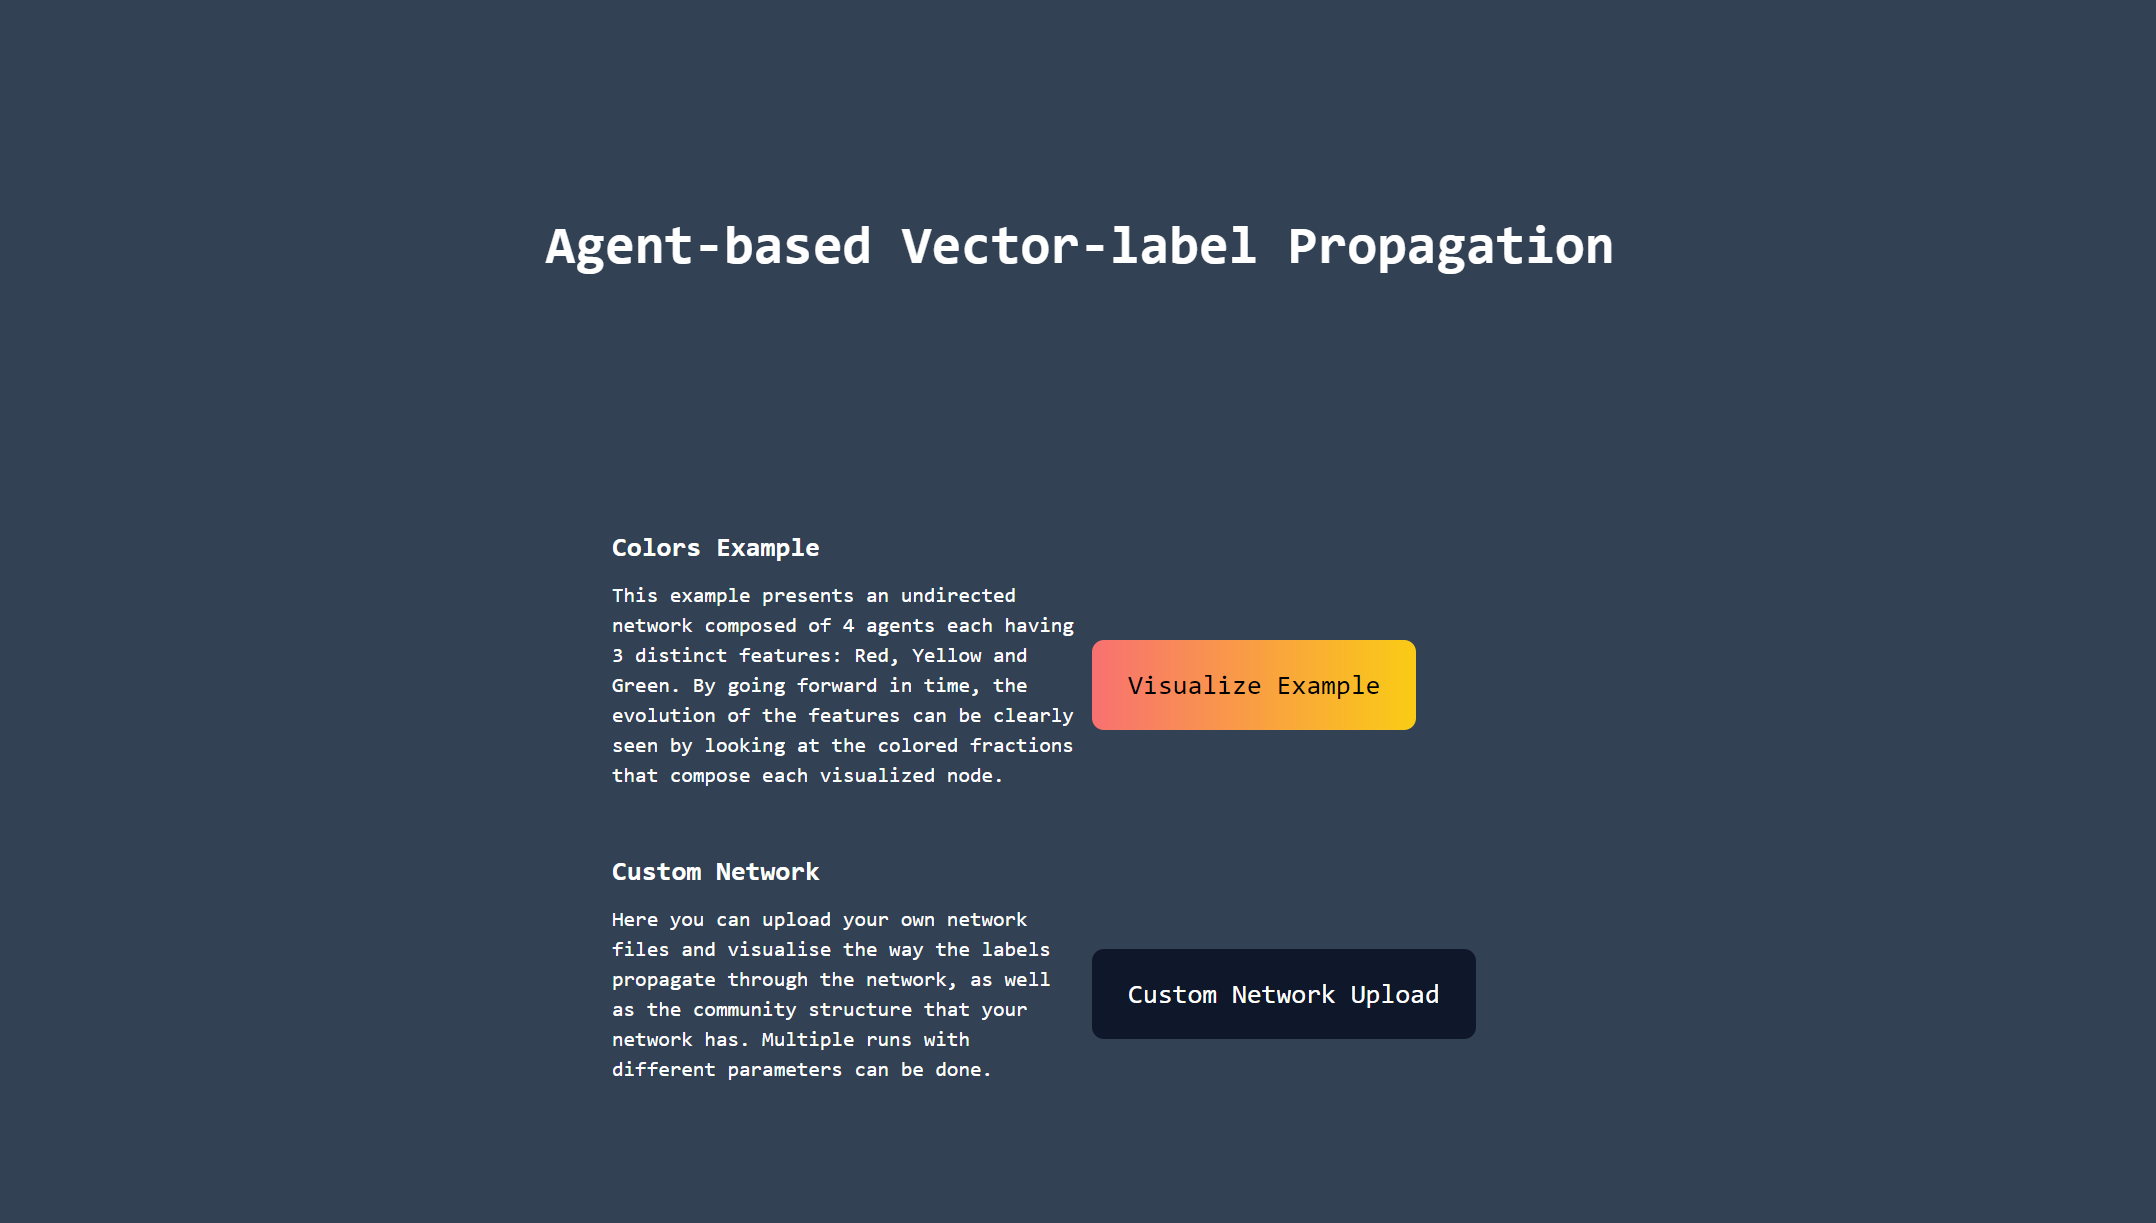
\includegraphics[width=0.9\linewidth,keepaspectratio]{paginaprincipale}
			\caption{Pagina Principale}
			\end{figure}
			\end{center}

			\subsubsection{Esempio Colori}

			La pagina dell'esempio colori, che si può raggiungere premendo il bottone "Visualize Example" vicino a "Colors Example" sulla pagina principale, ha tutte le funzionalità dell'applicazione, dimostrate su un semplice esempio di grafo non diretto con 4 nodi e 3 archi. In questo esempio si può vedere il modo in cui le etichette si propagano ad ogni iterazione attraverso i colori. 


			\begin{center}
			\begin{figure}[H]
			\centering
			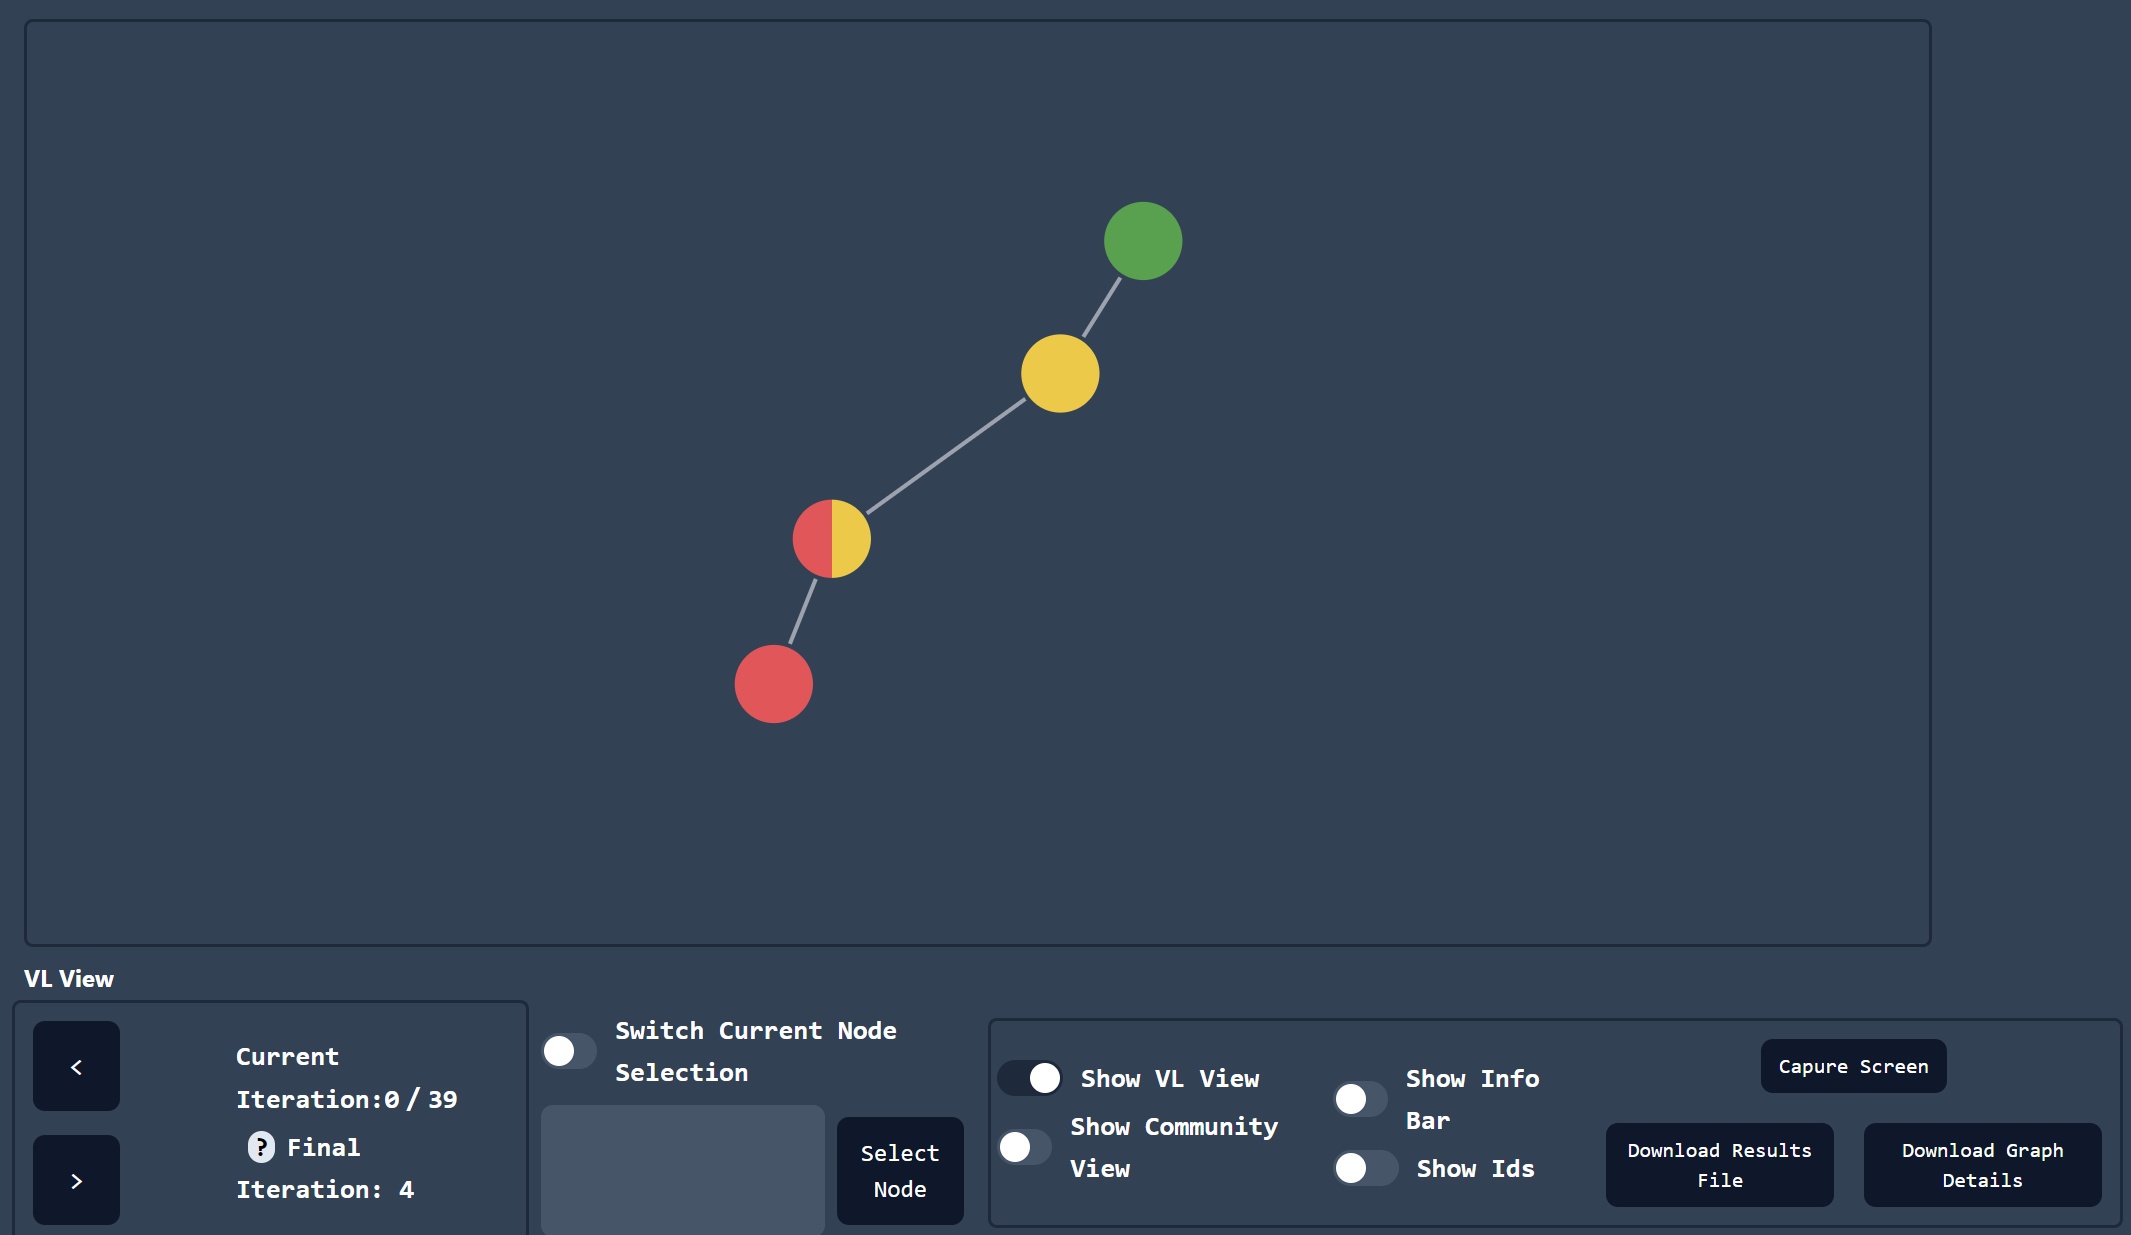
\includegraphics[width=0.9\linewidth,keepaspectratio]{colorsexample}	
			\caption{Esempio Colori}
			\end{figure}
			\end{center}
			I componenti che compongono l'interfaccia di visualizzazione della rete sono:
			\begin{itemize}
			\item \textbf{La bara di controllo} 

			Questo componente contiene tutte le modalità che si possono usare per controllare la visualizzazione della rete. 

			Iniziando da sinistra e andando verso destra, la bara di controllo contiene per prima cosa un rettangolo con dei tasti per controllare l'iterazione corrente che viene visualizzata, assieme alla iterazione che viene considerata finale dall'algoritmo (nel caso dell'esempio colori, il parametro $p$ viene fissato a 0.1). 
			
			
			\begin{center}
			\begin{figure}[H]
			\centering
			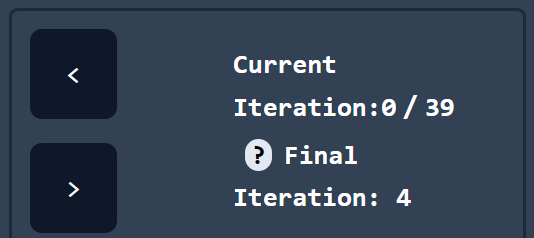
\includegraphics[width=0.8\linewidth,keepaspectratio]{iterationcontrol}
			\caption{Controlli Iterazione}
			\end{figure}
			\end{center}

			La seconda parte della bara di controllo viene utilizzata per cambiare il modo di selezione nodo e per cercare un nodo specifico nella rete. Se si preme il tasto per cambiare il modo di selezione nodo, si può selezionare un secondo nodo, in modo che, ulteriormente, si possono comparare i vettori di etichette dei due nodi. La bara di ricerca di un nodo specifico diventa molto utile nel caso in cui la rete utilizzata ha molti nodi e quindi dove la selezione del nodo dalla rete diventa difficile. 
			
			\begin{center}
			\begin{figure}[H]
			\centering
			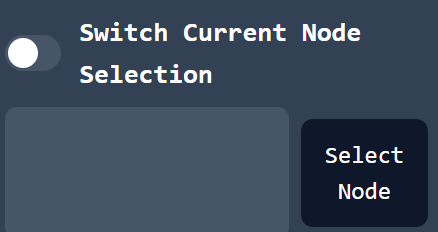
\includegraphics[width=0.8\linewidth,keepaspectratio]{nodeselection}
			\caption{Controlli Selezione Nodo}
			\end{figure}
			\end{center}

			L'ultima parte della bara di controllo contiene alcuni controlli per cambiare il layout di visualizzazione e alcuni tasti per: catturare la configurazione corrente dell'applicazione, scaricare il file dei risultati, scaricare il file contenente i dettagli del grafo e scaricare un file contenente la comparazione tra due nodi selezionati (tasto attivo solo nel caso in cui sono stati selezionati già due nodi). 

			Le opzioni per cambiare la configurazione dell'applicazione sono: Show VL View (che viene utilizzato per nascondere o per visualizzare la View che presenta graficamente la configurazione dei vettori di etichette), Show Community View (che viene utilizzato per nascondere o per visualizzare la View che presenta graficamente la divisione in comunità della rete), Show Info Bar (che viene utilizzato per nascondere e far comparire la bara laterale che presenta le informazioni sulla rete, o sui nodi selezionati) e Show Ids (che viene utilizzato per nascondere o per visualizzare gli ID all'interno di ogni nodo in una View). 

			\begin{center}
			\begin{figure}[H]
			\centering
			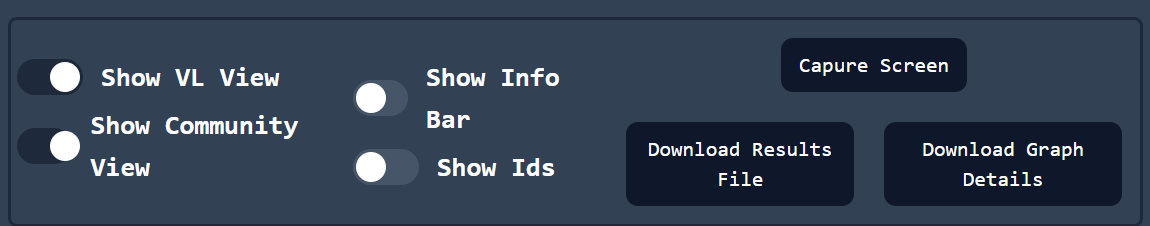
\includegraphics[width=0.9\linewidth,keepaspectratio]{viewcontrol}
			\caption{Controlli Vista}
			\end{figure}
			\end{center}

\pagebreak
			Il formato del file JSON in cui i dettagli della rete viene esportata e il seguente:
\begin{lstlisting}
{
	"directed": ...,
	"multigraph": ...,
	"graph": 
	{
		"labels": [...],
		"diameter": ...,
		"communities": ...,
		"nodesCount": ...,
		"edgesCount": ...,
		"centrality": {
			"1": ...,
      			"2": ...,
			...
    		},
    		"timestamps": ...,
    		"finalTs": ...
  	},
	"nodes": 
	[
		{
			"community": ..., 
			"degree": ..., 
			"neigh": [...], 
			"id": ...
		},
		...
  	],
	"links": [
		{
			 "source": ..., 
			"target": ...
		},
		...
	]
}

\end{lstlisting}

\pagebreak

			Il formato del file JSON in cui la comparazione nodi viene esportata e il seguente:

			\begin{lstlisting}
{
	"node1": 
	{
		"community": ...,
		"degree": ...,
		"neigh": [...],
		"id": ...,
		"VL": [...],
		"betweenness_centrality": ...
	},
	"node2": 
	{
		"community": ...,
		"degree": ...,
		"neigh": [...],
		"id": ...,
		"VL": [...],
		"betweenness_centrality": ...
	},
	"cosineSimilarity": ...,
	"timestamp": ...
}
			\end{lstlisting}


\pagebreak
			\item \textbf{VL View} 

			La VL View rappresenta la vista che visualizza la rete dal punto di vista dei vettori delle etichette. Tutti i belonging coefficient sommano a 1 e quindi ogni etichetta viene rappresentata da un colore che occupa la percentuale specifica sul nodo (per esempio se un'etichetta su un nodo ha il belonging coefficient uguale a 0.5, allora il colore di quell'etichetta occuperà 50\% del nodo nella VL View). 
			
			\begin{center}
			\begin{figure}[H]
			\centering
			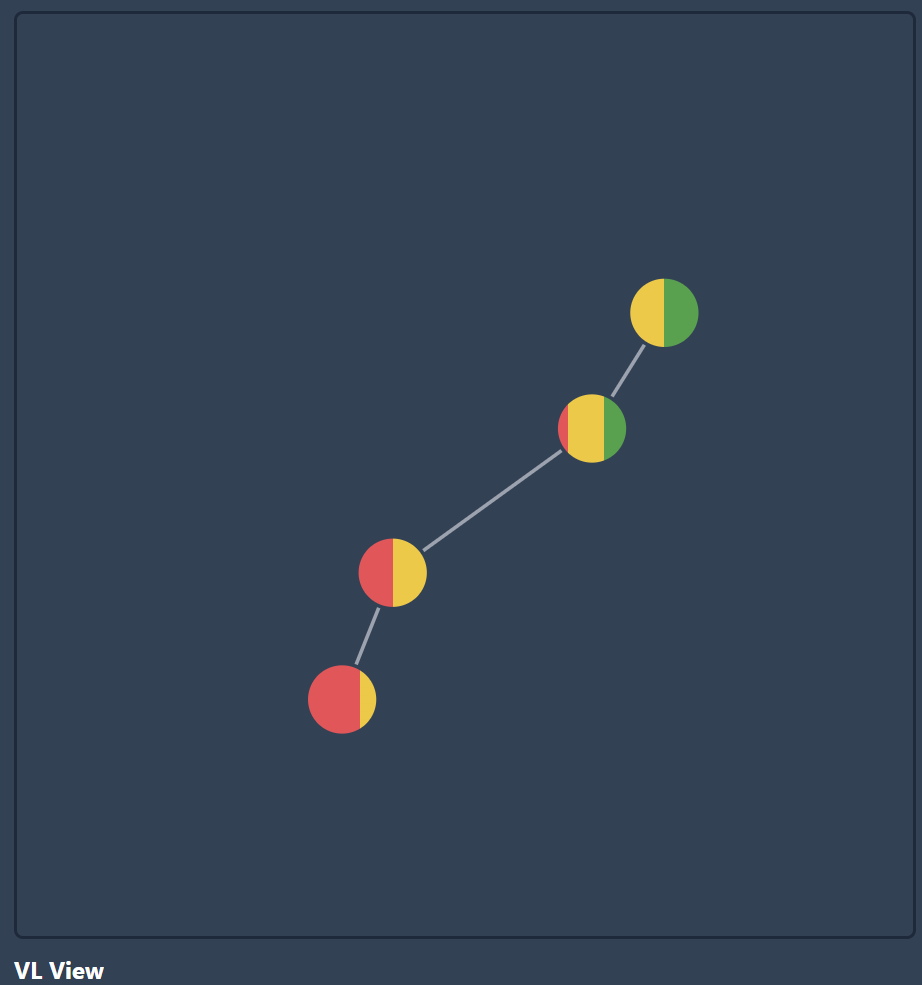
\includegraphics[width=0.9\linewidth,keepaspectratio]{vlview}
			\caption{Vista Vettori di etichette}
			\end{figure}
			\end{center}

			\begin{center}
			\begin{figure}[H]
			\centering
			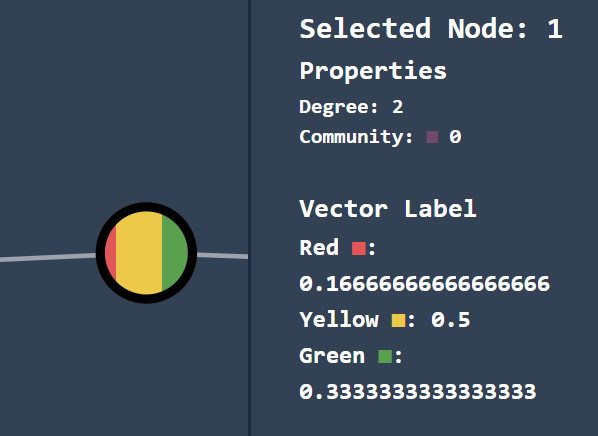
\includegraphics[width=0.8\linewidth,keepaspectratio]{vlrep}
			\caption{Un nodo nella vista Vettori di etichette}
			\label{fig:vlrep}
			\end{figure}
			\end{center}

			Nella figura \ref{fig:vlrep} si può vedere come ad ogni etichetta viene associato un colore vicino al suo nome, e un valore che rappresenta il belonging coeffcient di quell'etichetta per il nodo selezionato, all'iterazione corrente. 

			I colori dentro il nodo sono rappresentati in questo modo siccome l'etichetta \textbf{Red} ha un belonging coefficient di 0.16\dots (quindi 16.6\dots\% del nodo viene riempito col colore rosso), l'etichetta \textbf{Yellow} ha un belonging coefficient di 0.5 (quindi 50\% del nodo viene riempito col colore giallo) e l'etichetta \textbf{Green} ha un belonging coefficient di 0.33\dots (quindi 33.3\dots\% del nodo viene riempito col colore verde).

\pagebreak

			\item \textbf{Community View} 

			La Community View rappresenta la vista che visualizza la rete dal punto di vista delle comunità che compongono la rete. I nodi che si trovano nella stessa comunità avranno lo stesso colore, in modo da identificare facilmente i nodi appartenenti alla stessa comunità dal punto di vista strutturale. La comunità di ogni nodo può essere conosciuta dalle informazioni specifiche di ogni nodo, quando esso viene selezionato. 

			\begin{center}
			\begin{figure}[H]
			\centering
			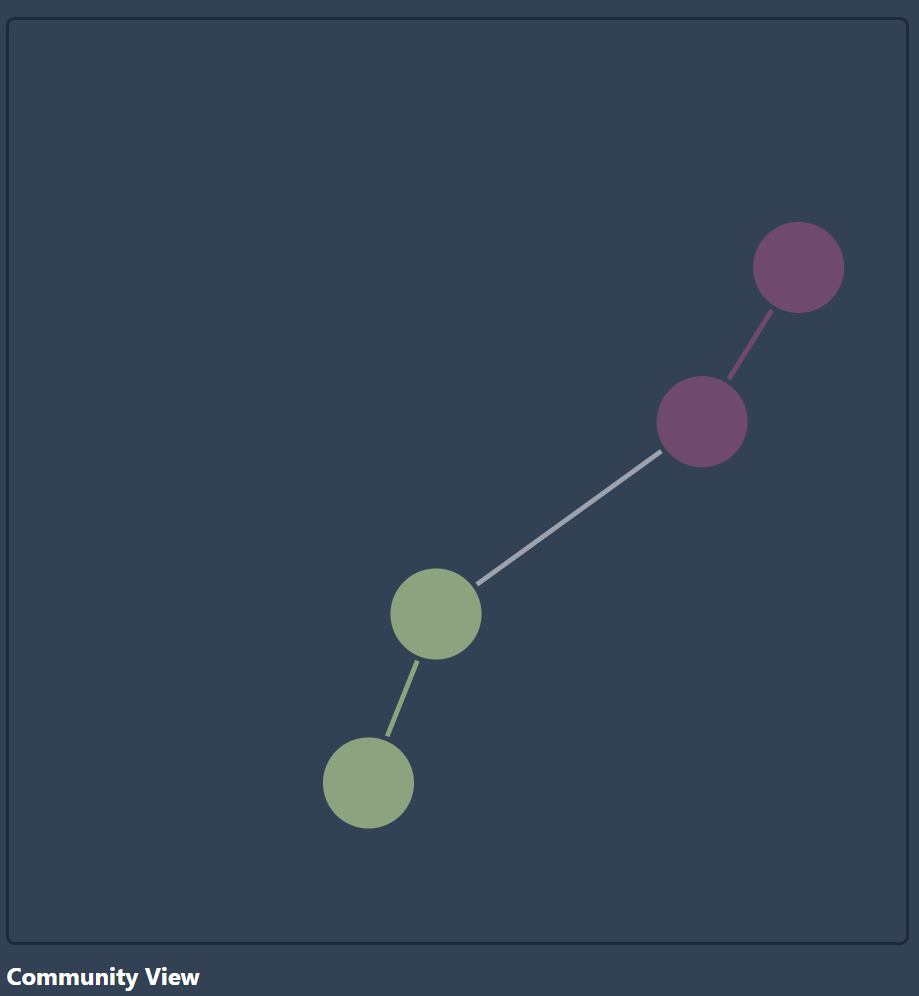
\includegraphics[width=0.9\linewidth,keepaspectratio]{comview}
			\caption{Vista comunità}
			\end{figure}
			\end{center}

\pagebreak

			\item \textbf{Info Bar} 

			La Info Bar visualizza, nel caso nessun nodo viene selezionato, le informazioni generali riguardanti la rete, come tipo di rete, numero di nodi, numero di archi e diametro. Nel caso in cui un nodo viene selezionato, la bara delle informazioni mostra il grado di quel nodo, la comunità appartenente, assieme al suo colore e il vettore delle etichette coi belonging coefficient di ogni etichetta, assieme al colore dell'etichetta. Nel caso in cui due nodi vengono selezionati, ci saranno due bare di informazioni che mostrano le stesse informazioni di prima per entrambi i nodi. 

			\begin{center}
				\begin{figure}[H]
				\centering
				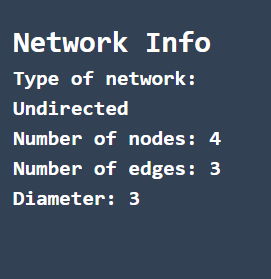
\includegraphics[width=0.4\linewidth]{infobargeneral}
				\caption{Barra Informazioni senza un nodo selezionato}
				\end{figure}
				\begin{figure}[H]
				\centering
				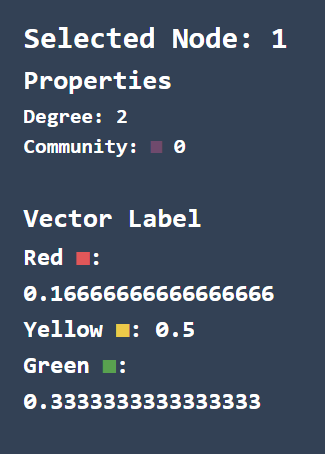
\includegraphics[width=0.4\linewidth]{infobar1}
				\caption{Barra Informazioni con un solo nodo selezionato}
				\end{figure}
				\begin{figure}[H]
				\centering
				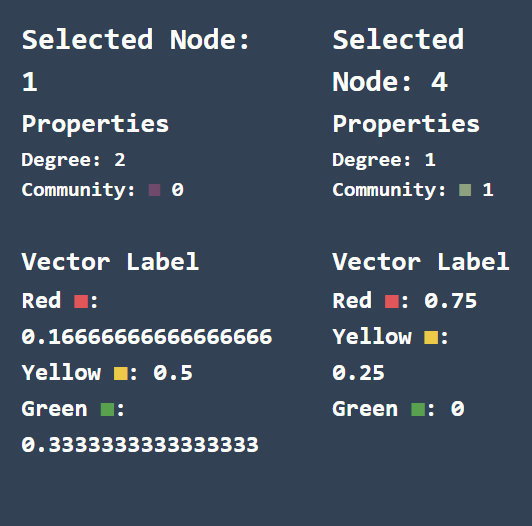
\includegraphics[width=0.6\linewidth]{infobar2}
				\caption{Barra Informazioni con due nodi selezionati}
				\end{figure}
			\end{center}
			\end{itemize}
			
			\subsubsection{Pagina Caricamento Reti Sociali Personalizzate}
			Nel caso della pagina di upload delle reti sociali personalizzate, l'utente può caricare i suoi dataset personali, formattati in un formato descritto nella pagina stessa, e visualizzare i risultati di AVPRA sulla sua rete. 

			L'utente ha la possibilità di personalizzare diverse opzioni riguardanti l'interpretazione dei dati e i parametri con cui l'algoritmo sarà eseguito. 

			I file riguardanti la rete che l'utente può caricare sull'applicazione sono i seguenti:

			\begin{itemize}
				\item Il file degli archi 
				
				Questo file dev'essere un file .csv col seguente formato: 

				\begin{equation}
				\begin{aligned}
				\dots \\
				nodo_1\ nodo_2\ \{ p \} \\
				\dots
				\end{aligned}
				\end{equation}

				Questo formato mostra che il $nodo_1$ e collegato al $nodo_2$ e che l'arco ha il peso $p$. Il peso è un parametro opzionale e quindi il file può essere definito anche nel seguente modo: 

				\begin{equation}
				\begin{aligned}
				\dots \\
				nodo_1\  nodo_2 \\
				nodo_2\  nodo_4 \\
				\dots
				\end{aligned}
				\end{equation}				

				\item Il file dei vettori delle etichette con cui i nodi vengono inizializzati. 

				Questo file dev'essere un file .csv col seguente formato: 

				\begin{equation}
				\begin{aligned}
				b_1(l_1);\ b_1(l_2);\ \dots;\ b_1(l_k) \\
				b_2(l_1);\ b_2(l_2);\ \dots;\ b_2(l_k) \\
				b_3(l_1);\ b_3(l_2); \dots;\ b_3(l_k) \\
				\dots
				\end{aligned}
				\end{equation}
				
				In questo caso $b_1, b_2, b_3, \dots$ sono le funzioni del coefficiente d'appartenenza dei nodi $1, 2, 3, \dots$ e $l_1, l_2, \dots, l_k$ sono le etichette della rete. I valori di ogni riga devono sommare a 1. 
				

				\item Il file dei nomi delle etichette
				
				Questo file dev'essere un file .csv col seguente formato: 

				\begin{equation}
				l_1;\ l_2;\ l_3;\ l_4;\ \dots
				\end{equation}

				\item Il file dei colori con cui vengono rappresentate le etichette. 

				Questo file dev'essere un file .csv che ha il seguente formato: 

				\begin{equation}
				hex_1;\ hex_2; \dots
				\end{equation}
				In questo formato $hex_1, hex_2, \dots$ sono i codici esadecimali dei colori con cui saranno rappresentate le etichette $l_1, l_2, \dots$ nella visualizzazione. 

				Un esempio del formato di questo file è: 

				\begin{equation}
				\#433A3F;\ \#404A56;\ \#3D5A6C;\ \#58827E;\ \#659687; \dots
				\end{equation}
			\end{itemize}
			
			Le opzioni che l'utente può scegliere sono le seguenti:
			
			\begin{itemize}
				\item Grafo diretto o non diretto 

				Quest'opzione permette all'utente di scegliere se il grafo costruito dal file degli archi viene interpretato come un grafo diretto o non diretto.

				\item Propagazione delle etichette dai predecessori o successori 

				Quest'opzione permette all'utente di scegliere se la propagazione delle etichette viene influenzata dagli nodi vicini entranti o dagli nodi vicini uscenti. Nel caso in cui il grafo viene interpretato come un grafo non diretto, quest'opzione non è disponibile.

				\item Negligibly Threshold / Soglia di trascuramento

				Quest'opzione permette all'utente di scegliere il valore del parametro negligibly threshold associato all'algoritmo, da cui dipende l'iterazione finale dell'algoritmo.

				\item Numero di iterazioni 

				Quest'opzione permette all'utente di scegliere il numero di iterazioni per cui l'algoritmo sarà eseguito.

				\item Formula per il peso nella funzione di aggiornamento 

				Quest'opzione permette all'utente di scegliere una formula (dipendente dal numero di vicini del nodo) per i pesi nella funzione di aggiornamento dell'algoritmo AVPRA.


				\begin{equation}
				\label{eqn:weightformula}
				VL_i [l] (t) = (1-w) VL_i [l] (t-1) + w \sum_{j \in \Gamma(i)} VL_j [l](t-1)
				\end{equation}

				Nella formula \ref{eqn:weightformula}, il peso che viene scelto dall'utente è $w$. Se l'utente non sceglie un peso personalizzato per $w$, allora $w=\frac{1}{k+1}$, dove $k$ è il numero di vicini del nodo $i$.

			\end{itemize}
			
			\subsubsection{Esempio Personalizzato}

			Nel caso dell'esempio personalizzato, l'interfaccia utente e praticamente uguale all'interfaccia presente nell'Esempio Colori, con qualche piccola differenza data dalle opzioni che l'utente ha scelto nella fase di caricamento della rete.

			\paragraph*{La bara di informazioni} si comporta nello stesso modo della bara di informazioni dell'Esempio Colori, ma offre più informazioni generali riguardo la rete caricata sull'applicazione.
			
			\begin{center}
				\begin{figure}[H]
				\centering
				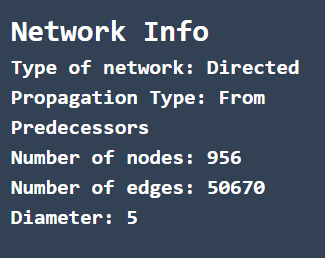
\includegraphics[width=0.5\linewidth]{infobargeneralcustom}
				\caption{Barra Informazioni Generale per una rete diretta e con propagazione delle etichette da predecessori}
				\end{figure}
				\begin{figure}[H]
				\centering
				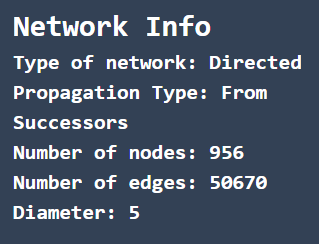
\includegraphics[width=0.5\linewidth]{infobargeneralcustomdirectedsuccessors}
				\caption{Barra Informazioni Generale per una rete diretta e con propagazione delle etichette da successori}
				\end{figure}
				\begin{figure}[H]
				\centering
				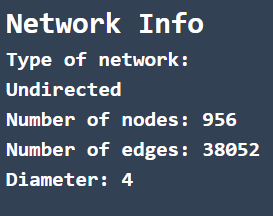
\includegraphics[width=0.5\linewidth]{infobargeneralcustomundirected}
				\caption{Barra Informazioni Generale per una rete non diretta}
				\end{figure}
			\end{center}

\pagebreak

			\paragraph*{La barra di controllo} subisce modifiche solo nella sezione di Controlli Iterazione. In questo caso, il numero massimo delle iterazioni viene sostituito col numero di iterazioni scelto dall'utente durante il caricamento della rete, e l'iterazione finale cambia in modo che il numero d'ordine mostrato sia l'iterazione dove avviene la condizione di terminazione.

			\begin{center}
				\begin{figure}[H]
				\centering
				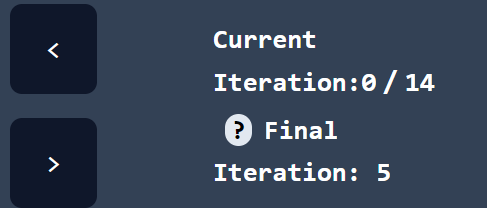
\includegraphics[width=0.5\linewidth]{iterationcontrolcustom}
				\caption{Controlli Iterazione per reti personalizzate}
				\end{figure}
			\end{center}
\chapter{Sviluppi Futuri}

	\section{Comunità}
	
	La sezione riguardante le comunità può essere estesa in modo da permettere l'utilizzo di un modello di Machine Learning per poter riconoscere le comunità rispetto ai vettori di etichette ad ogni iterazione, invece della struttura.

	\section{Deployment}

	Una delle cose che vanno fatte nel futuro e la pubblicazione dell'applicazione web in modo che gli utenti possano utilizzare l'applicazione in modo semplice.

	Il frontend, che e stato sviluppato con l'aiuto di Next.js, può essere facilmente distribuito attraverso un server Node.js basato, per esempio, su \textbf{AWS EC2} o un \textbf{DigitalOcean Droplet} \cite{nextjsdep}. Un altro modo molto semplice per la distribuzione del frontend è attraverso \textbf{Firebase Hosting} di \textbf{Google Firebase}, che dopo qualche semplice configurazione, permette la pubblicazione dell'applicazione web in modo gratuito (entro certi limiti d'utilizzo) \cite{firebasehosting}. 

	Il backend, sviluppato usando Flask e scritto in Python, può essere distribuito usando le \textbf{Google Cloud Functions} di \textbf{Google Firebase}, in modo che ogni endpoint sia collegato a una funzione in cloud che può essere chiamata dal frontend \cite{googlecloudfunctions}.

\chapter{Conclusioni}

%
%			BIBLIOGRAFIA
%
\begin{thebibliography}{0}
%
\bibitem{mapequationsite}
https://www.mapequation.org/infomap/

\bibitem{mapequationnavigatorsite}
https://www.mapequation.org/navigator/

\bibitem{snaintro}
https://towardsdatascience.com/social-network-analysis-from-theory-to-applications-with-python-d12e9a34c2c7

\bibitem{gregory}
Gregory, S.: Finding overlapping communities in networks by label propagation.
New journal of Physics 12(10), 103018 (2010)

\bibitem{avpra}
Valerio Bellandi, Paolo Ceravolo, Ernesto Damiani, and Samira Maghool: Agent-based Vector-label Propagation for Explaining Social Network Structures. In: Springer Verlag (Lecture Notes in Communications in Computer and Information Science (CCIS)) (2022)

\bibitem{raghavan}
Raghavan, U.N., Albert, R., Kumara, S.: Near linear time algorithm to detect
community structures in large-scale networks. Physical review E 76(3), 036106
(2007)

\bibitem{componentireact}
https://it.reactjs.org/docs/react-component.html

\bibitem{tipicomponenti}
https://it.reactjs.org/docs/components-and-props.html

\bibitem{statoreact}
https://it.reactjs.org/docs/state-and-lifecycle.html

\bibitem{jsxreact}
https://it.reactjs.org/docs/introducing-jsx.html

\bibitem{hooksreact}
https://it.reactjs.org/docs/hooks-intro.html

\bibitem{typescript}
https://www.typescriptlang.org/

\bibitem{typescripthandbook}
https://www.typescriptlang.org/docs/handbook/typescript-in-5-minutes-func.html

\bibitem{nextjs}
https://nextjs.org/learn/foundations/about-nextjs/what-is-nextjs

\bibitem{d3js}
https://d3js.org/

\bibitem{katex}
https://www.npmjs.com/package/katex

\bibitem{tailwindcss}
https://tailwindcss.com/

\bibitem{flaskforeword}
https://flask.palletsprojects.com/en/2.1.x/foreword/

\bibitem{flask}
https://flask.palletsprojects.com/en/2.1.x/

\bibitem{sympy}
https://www.sympy.org/en/index.html

\bibitem{cdlib}
https://cdlib.readthedocs.io/en/latest/

\bibitem{nextjsdep}
https://nextjs.org/docs/deployment

\bibitem{firebasehosting}
https://firebase.google.com/docs/hosting

\bibitem{googlecloudfunctions}
https://cloud.google.com/functions
%
\end{thebibliography}
% 
\end{document}


 
